\documentclass{article}
\usepackage{enumitem,graphicx,titling,units,braket,amsthm, amsmath,amssymb,mathtools,textcomp,tikz,pgfplots,listings,hyperref, physics, listings, color}

\newcommand\numberthis{\addtocounter{equation}{1}\tag{\theequation}}
\allowdisplaybreaks[1]

\makeatletter
\def\myitem{%
   \@ifnextchar[ \@myitem{\@noitemargtrue\@myitem[\@itemlabel]}}
\def\@myitem[#1]{\item[#1]\mbox{}\\\hspace*{\dimexpr-\labelwidth-\labelsep}}
\makeatother

\newtheorem{theorem}{Theorem}
\newtheorem{corollary}[theorem]{Corollary}
\newtheorem{conjecture}[theorem]{Conjecture}

\lstset{
	tabsize=4,
	rulecolor=,
	language=python,
        basicstyle=\scriptsize,
        upquote=true,
        aboveskip={1.5\baselineskip},
        columns=fixed,
        showstringspaces=false,
        extendedchars=true,
        breaklines=true,
        prebreak = \raisebox{0ex}[0ex][0ex]{\ensuremath{\hookleftarrow}},
        frame=single,
        showtabs=false,
        showspaces=false,
        showstringspaces=false,
        identifierstyle=\ttfamily,
        keywordstyle=\color[rgb]{0,0,1},
        commentstyle=\color[rgb]{0.133,0.545,0.133},
        stringstyle=\color[rgb]{0.627,0.126,0.941},
}

\begin{document}
	\setlength{\droptitle}{-10em}
	\title{Homework 2}
	\author{Andrew Lei\\Arizona State University}
	\maketitle
	
	\section{Part 1}
	\noindent
	\textbf{Question 1}
	\begin{figure}[h]
		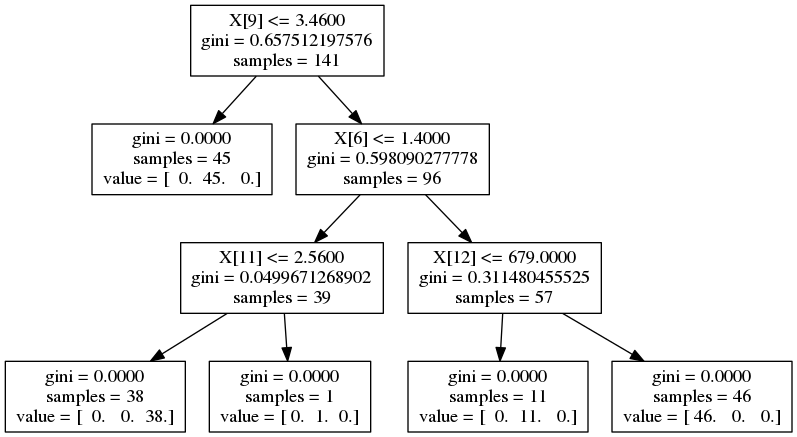
\includegraphics[scale=0.5]{gini_tree.png}
		\caption{Decision tree constructed from wine training data using Gini impurity for splitting criterion}
	\end{figure}
	\par
	It seems all samples with a low value for the tenth attribute (X[9] indexing from zero), intensity, fall into Category 2, which also makes up most (more than 80\%) of the Category 2 samples. 
	\par
	Another important attribute split on is the seventh attribute, flavanoids, where, if high in intensity, lower values fall into Category 3, and higher values fall into either Categories 1 or 3 (mostly the first).
	\par
	Finally, there's a split on proline (attribute 13) for samples high in intensity and flavanoids. Lower values are Category 2, and higher values are Category 1 (all Category 1 samples were high in intensity, flavanoids, and proline). 
	\par
	There is a split on the twelfth attribute (OD280/OD315 of diluted wines), but one of the two leaves only contains a single element, so it probably is not significant.
	\par 
	Accuracy was 100\%.
	
	\newpage
	\noindent
	\textbf{Question 2}
	\begin{figure}[h]
		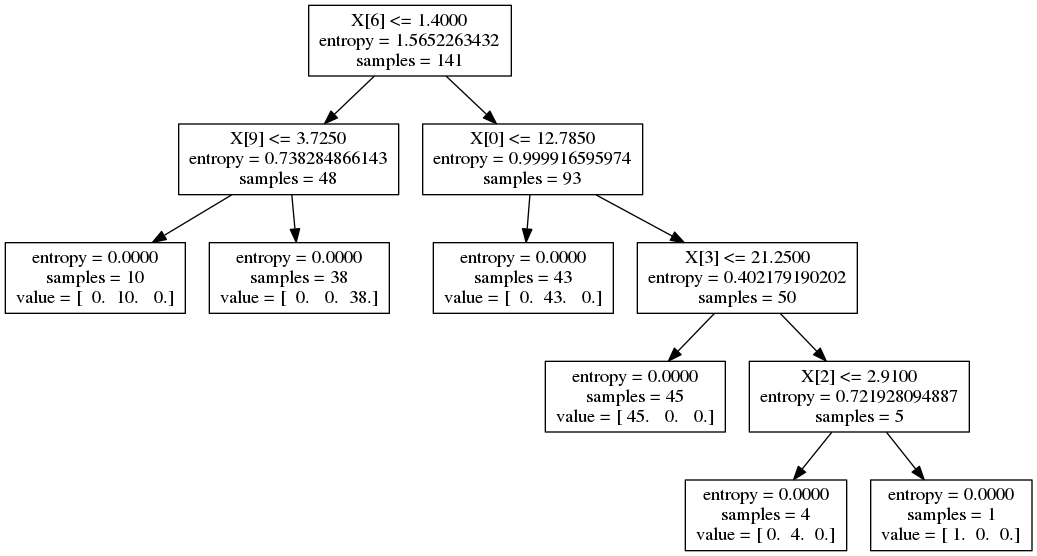
\includegraphics[scale=0.4]{entropy_tree.png}
		\caption{Decision tree constructed from wine training data using entropy gain for splitting criterion}
	\end{figure}
	\par 
	This tree also splits on flavanoids and intensity, but in the opposite order. However, there is still the same pattern; samples low in intensity are Category 2, while samples high in intensity and but low in flavanoids tend to be Category 3.
	\par
	The rest of the splitting is different. After splitting on flavanoids (high), the next split is on alcohol content. Category 2 has low alcohol content while Category 1 has high. There are a few more splits, but they have very few samples, so are probably not significant.
	\par 
	Accuracy was 100\%.\\\\
	
	\noindent
	\textbf{Question 3}
	\par 
	Accuracy for Gini was 94.3\% while the accuracy for entropy was 85.7\%. It seems entropy performed significantly worse because it was overfit compared to the Gini decision tree. There are six leaves in the entropy tree but only five in the Gini tree. Further, the tree itself is one layer taller.
	\par 
	The following is the code I used for the first part. You can find it on my GitHub at 
	\newpage
	\begin{lstlisting}[language=python]
#! /usr/bin/env python

import pandas as pd
import matplotlib.pyplot as plt
import numpy as np
import statsmodels.formula.api as sm
from sklearn.tree import DecisionTreeClassifier
from sklearn import tree

# Read training data
train = pd.read_csv('wine.trainingdata.txt')
# First column is label (i.e., y), rest go to X
(y_train, X_train) = (train.ix[:,0], train.ix[:,1:])

# Question 1
# Train decision tree classifier using Gini impurity
clf_gini = DecisionTreeClassifier(criterion = 'gini')
clf_gini.fit(X_train, y_train)
# Print training score for tree with Gini criterion
print 'Gini criterion training score: ', clf_gini.score(X_train, y_train)
# Save tree
tree.export_graphviz(clf_gini, out_file='gini_tree.dot')

# Question 2
# Train decision tree classifier using entropy
clf_entropy = DecisionTreeClassifier(criterion = 'entropy')
clf_entropy.fit(X_train, y_train)
# Print training score for tree with entropy
print 'Entropy criterion training score: ', clf_entropy.score(X_train, y_train)
# Save tree
tree.export_graphviz(clf_entropy, out_file='entropy_tree.dot')

# Question 3
# Read testing data
test = pd.read_csv('wine.TestData.txt')
(y_test, X_test) = (test.ix[:,0], test.ix[:,1:])
# Print training scores
print 'Gini criterion testing score: ', clf_gini.score(X_test, y_test)
print 'Entropy criterion testing score: ', clf_entropy.score(X_test, y_test)
	\end{lstlisting}
	\newpage
	
	\section{Part 2}
	\par 
	There are 12 `Yes' samples and 8 `No' samples for `Electronics' (60 and 40 per cent, respectively), so the initial entropy is 
	\begin{align*}
		S_0 &= -0.4\log_2 0.4 - 0.6\log_2 0.6\\
		&\approx 0.971
	\end{align*}
	\par
	Four of ten males and four of ten females answered `No' for `Electronics'. This is the same proportion as the overall population; so entropy from splitting on population here does not change.
	\par
	I assume we must do binary splits, in which case it makes sense to group together for car owners those who answered `No' 50\% or more as one branch of the split, and those who answered unanimously `Yes' as another.
	\par 
	Three of five sedan owners answered `No' (60\%). Three of six truck owners answered `No' (50\%). Two of four van owners answered `No' (50\%). Combined, this is 8 out of 15, with entropy
	\begin{align*}
		S &= -\frac{8}{15}\log\frac{8}{15} -\frac{7}{15}\log\frac{7}{15}\\
		&\approx 0.997
	\end{align*}
	Meanwhile, four of four sports car owners answered `Yes' (100\%), and the sole medium car owner answered `Yes' (100\%), giving an entropy of
	\begin{align*}
		S &= -1\log_2 1 - 0\log_2 0\\
		&= 0
	\end{align*}
	The average entropy (and gain) is then\footnote{In class it was stated that a simple average instead of a weighted one should be used, but this would puzzlingly lead to a split where a single `Yes' element is a branch has a lower entropy than multiple if the latter leads to a split closer to 50-50. For this reason, and because several examples I read seem to do this, I decided to use a weighted average.}
	\begin{align*}
		S_1 &= \frac{5\cdot 0 - 15\cdot\left(\frac{8}{15}\log\frac{8}{15} + \frac{7}{15}\log\frac{7}{15}\right)}{20}\\
		&\approx 0.748\\
		\Delta S &= S_1 - S_0\\
		&\approx -0.223
	\end{align*}
	\par 
	Four of four married answered `Yes' (100\%). Three of eight (37.5\%) single answered `No'. Finally, four of eight divorced answered `No'. We can either group single and married or single and divorced. If the former, we get 9 of 12 answering `Yes' and then
	\begin{align*}
		S &= -\frac{3}{4}\log_2\frac{3}{4}-\frac{1}{4}\log_2\frac{1}{4}\\
		&= 0.811
	\end{align*}
	Meanwhile, entropy for the divorced can be seen by inspection to be one, and the weighted average is then clearly greater than $0.748$. Grouping divorced and single, 7 of 16 (43.75\%) answered `No' and hence
	\begin{align*}
		S &= -\frac{7}{16}\log_2\frac{7}{16} - \frac{9}{16}\log_2\frac{9}{16}\\
		&= 0.989
	\end{align*}
	While the married entropy is zero. And so the average entropy (and gain) is
	\begin{align*}
		S_1 &= \frac{4\cdot 0 - 16\cdot\left(\frac{7}{16}\log_2\frac{7}{16} + \frac{9}{16}\log_2\frac{9}{16}\right)}{20}\\
		&\approx 0.791\\
		\Delta S &= S_1 - S_0\\
		&\approx -0.180
	\end{align*}
	\par 
	Hence we split on vehicle. Sports car and medium immediately terminate on `Yes', and since two of those were male and three female, it should be reasonable to assume that the entropy values do not change significantly for the remaining eight males and seven females (four of eight and four of seven, respectively, answer `No').
	\par 
	So clearly we must either split on marital status or further on vehicle type.
	\par 
	Note that of the remaining, two of two married answered `Yes' (100\%), three of six single answered `No' (50\%), and five of seven divorced answered `No' (71.4\%). We can either group together the first two or the latter two. If grouping married and single, five of eight (62.5\%) answer `Yes', and the two entropies we get are
	\begin{align*}
		S &= -\frac{5}{8}\log_2\frac{5}{8}-\frac{3}{8}\log_2\frac{3}{8}\\
		&= 0.954\\
		S &= -\frac{5}{7}\log_2\frac{5}{7}-\frac{2}{7}\log_2\frac{2}{7}\\
		&= 0.863
	\end{align*}
	\par
	But if we group together single and divorced, we have instead 8 of 13 `Yes', married with entropy zero, and non-married with entropy
	\begin{align*}
		S &= -\frac{8}{13}\log_2\frac{8}{13}-\frac{5}{13}\log_2\frac{5}{13}\\
		&= 0.961
	\end{align*}
	\par
	And average entropy
	\begin{align*}
		S_2 &= \frac{-13\cdot\left(\frac{8}{13}\log_2\frac{8}{13}+\frac{5}{13}\log_2\frac{5}{13}\right)}{15}\\
		&\approx 0.833
	\end{align*}
	Which is clearly less than both numbers from grouping married and single, and hence their weighted average must be greater than this. 
	\par
	Alternatively, we could split between sedan owners and the others, which have entropies of about 0.971 (because 60\% proportion, same as start) and 1, respectively; this should not be done, because their weighted average is greater than what we have here.
	\par 
	`Married' of course terminates, and we are let with `Single' and `Divorced'. One male and one female were eliminated, so four of seven and four of six, respectively, answer `No'. These correspond to entropies of 0.985 and 0.918.
	\par 
	Single and divorced have entropies of 1 (six samples) and 0.863 (seven), so it's quite simple to see splitting on this is superior to gender. Additionally, we could split on cars again.
	\par 
	Two of three van owners remaining answered `No'. Three of six truck owners answered `No'. Three of four sedan owners answered `No'. Combining van owners and sedan owners we the same proportions and thus entropies as splitting on marital status between single and divorced. Combining van owners and truck owners give five of nine answering `No' and three of four answering `Yes', corresponding to entropies
	\begin{align*}
		S &= -\frac{5}{9}\log_2\frac{5}{9} -\frac{4}{9}\log_2\frac{4}{9}\\
		&\approx 0.991\\
		S &= -\frac{3}{4}\log_2\frac{3}{4} -\frac{1}{4}\log_2\frac{1}{4}\\
		&\approx 0.811\\
	\end{align*}
	\par
	And the average entropy is then
	\begin{align*}
		S_3 &\approx \frac{9\cdot 0.991 + 4\cdot 0.811}{13}\\
		&\approx 0.936
	\end{align*}
	\par
	While the other possibilities have entropy
	\begin{align*}
		S_3 &\approx \frac{7\cdot 0.863 + 6\cdot 1}{13}\\
		&\approx 0.926
	\end{align*}
	\par 
	We could split on marital status or car, but I will split on marital status again here, between single and divorced.
	\par 
	If single, note that we cannot split on gender since all are 50-50 for `Yes' or `No'. So we must split on car type. From inspection, it's clear that vans (1/1 `Yes') will be grouped with trucks (2/3 `Yes') with sedans (2/2 `No') alone. This will then be split between vans and trucks (or females and males; all the males own trucks here), and no more distinctions can be made after splitting on that since all features will be identical (male, single, truck) and that leaf will return `Yes'.
	\par 
	If married, here are the remaining proportions: Sedans, 1/2 `No', trucks, 2/3 `No', vans, 2/2 `No', male, 2/3 `No', female, 3/4, `No'. It's clear if we split on vehicles and group sedans and vans, we will get the same as splitting by gender, but it's also clear that grouping sedans and trucks would be superior in lowering the entropy, so a split on vehicles between vans and non-vans is chosen. Now, the proportions are: male, 1/2 `No', female, 2/3 `No', sedan, 1/2 `No', truck, 2/3 `No'; the splitting is identical, but I will split on car type here again. Finally, for sedans, male is `No' and female is `Yes', while for trucks, female is `No' while male is `Yes'.
	\begin{figure}
		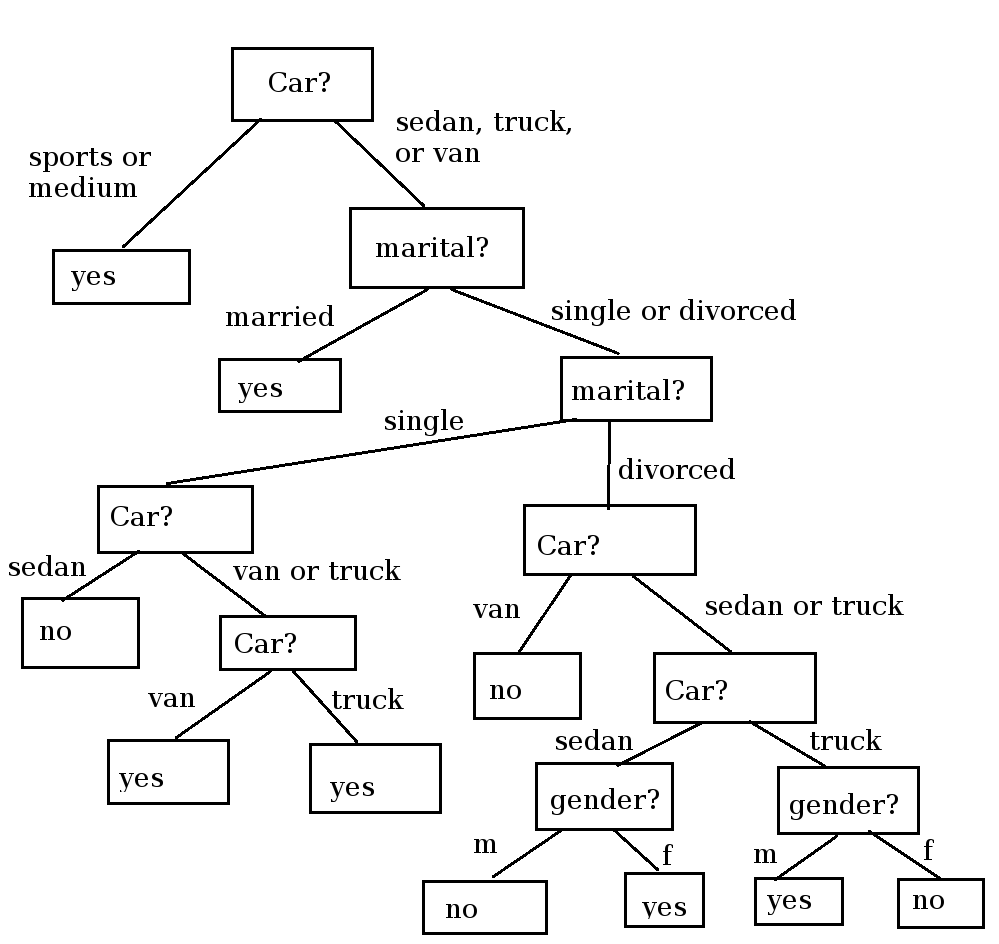
\includegraphics[scale=0.4]{part2tree.png}
		\caption{Tree for Part 2}
	\end{figure}
	
\end{document}